\documentclass{beamer}

\usepackage[size=custom,width=91.44,height=60.96,scale=1.12]{beamerposter}
\usepackage{graphicx}
\usepackage{url}
\usepackage{amsmath}
\usepackage{xfrac}
\usepackage{listings}
\usepackage{color}
\usepackage{caption}
\usepackage{subcaption}

\usetheme{Rochester}
\usecolortheme{UW}
\setbeamertemplate{headline}{}
\setbeamertemplate{navigation symbols}{}
\setbeamertemplate{footline}{}

\lstset{language=C,frame=single,breaklines=true,backgroundcolor=\color{white},basicstyle=\ttfamily}

\title[ShMemMC]{\Huge\textbf{Shared Memory Monte Carlo with MPI+MPI}}
\author{\normalsize Brian Cornille}
\institute{\normalsize University of Wisconsin-Madison, Department of Engineering Physics}

\begin{document}

\begin{frame}[t,fragile]{}

\begin{beamercolorbox}[center]{}
\maketitle
\end{beamercolorbox}

\begin{columns}[t,totalwidth=\textwidth]

\begin{column}{0.3\textwidth}

\begin{block}{\LARGE\textbf{Objectives}}
\begin{itemize}
\item Write a basic Monte Carlo transport code that uses good modular programming practices.
\item Demonstrate that Monte Carlo tallies can be implemented with
the MPI-3.0 shared memory infrastructure.
\item Investigate the computational trade-off of using shared memory tallies
in Monte Carlo calculations.
\end{itemize}
\end{block}

\begin{block}{\LARGE\textbf{Motivation}}
Extremely large Monte Carlo calculations are carried out on high performance computing (HPC) systems.
Message Passing Interface (MPI) is a common programming model that is utilized for the parallelism
in HPC environments.
In the context of Monte Carlo and MPI the geometry and tallies are usually repeated for each process,
while unique particles are transported on each process that contribute to the overall result.
However, for very large mesh tallies, the limits of available memory can be reached, especially
when computational nodes have many processors that the node's memory must be split between.
More efficient use of the resources on one node would suggest sharing the information on geometry
and tallies instead of repeating it.
For previous versions of the MPI standard this was not possible.
\begin{figure}
\begin{subfigure}[b]{0.49\textwidth}
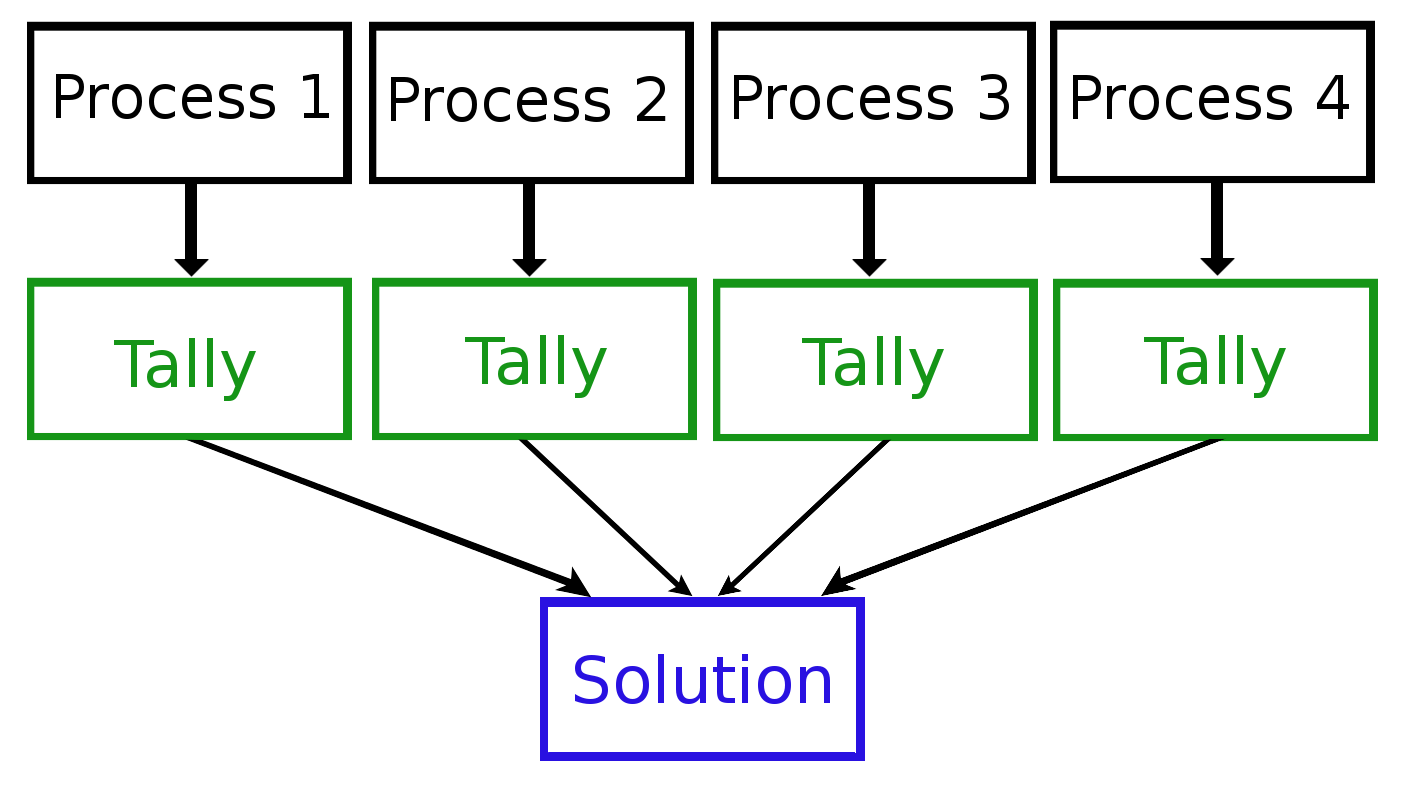
\includegraphics[width=\textwidth]{Distributed.png}
\caption{Distributed Memory}
\end{subfigure}
\begin{subfigure}[b]{0.49\textwidth}
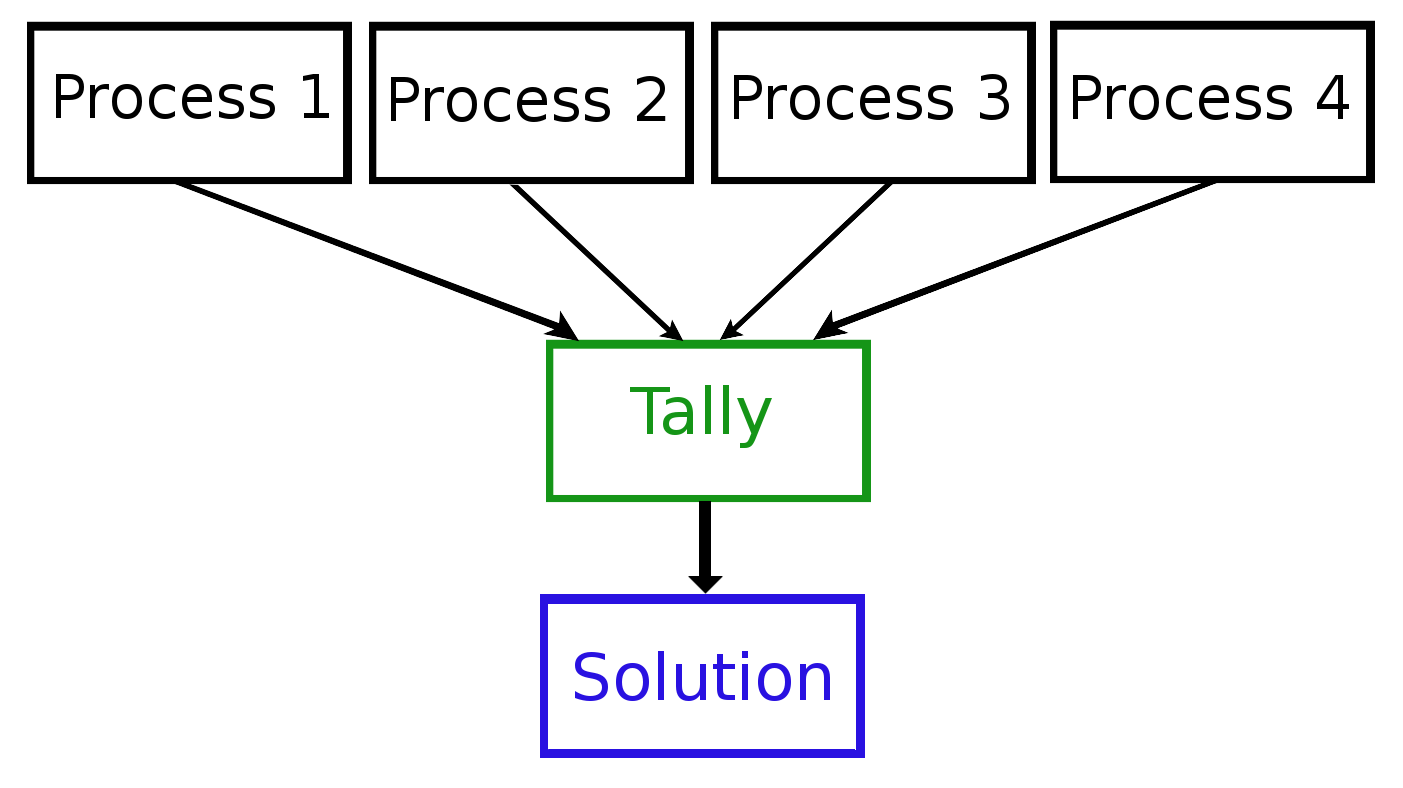
\includegraphics[width=\textwidth]{Shared.png}
\caption{Shared Memory}
\end{subfigure}
\caption{Distributed and shared memory models for parallel Monte Carlo calculations}
\end{figure}

The MPI-3.0 Standard allows for the allocation of shared memory regions for processes that share
physical memory space, such as those on a single compute node in a larger HPC cluster.
This allows for what is called an MPI+MPI hybrid parallel programming model (previously one would
have to do MPI+X, where X is some shared memory parallel programming model).
The capabilities and limitations of MPI-3.0 shared memory should be investigated for Monte Carlo
applications.
\end{block}

\end{column}

\begin{column}{0.310\textwidth}

\begin{block}{\LARGE\textbf{Pitfalls of Shared Memory Parallelism}}
When multiple processes have access to the same memory,
there is increased risk for programming error.
The main concern in this scenario is that each process has no way of knowing when or in what manner
other processes are accessing the same memory locations.
If safety precautions are not taken to ensure that data is always up-to-date when a process wants
to execute a save or load at some memory location,
then what is called a \textit{race condition} may occur.
If a race condition exists in a program,
then that program is very likely to produce incorrect results.
Furthermore, the results can vary from run to run due to minor inconsistencies in the order with
which processes may access the memory associated with the race condition.
The MPI-3.0 shared memory model does not automatically provide safety against
race conditions using basic load/save operations for the shared memory.
The MPI standard provides a safe way to add a numerical contribution to a shared memory location
with the MPI\_Accumulate function.
This function is ideal for the purpose of tallies in Monte Carlo calculations.
\end{block}

\begin{block}{\LARGE\textbf{Model Problem}}
\begin{columns}[c,totalwidth=\textwidth]
\begin{column}{0.6\textwidth}
The geometry is a single cell in the shape of a rhombicuboctahedron.
A rhombicuboctahedron has 26 faces, thus 26 planes are used for the cell definition.
A model material is used that has a mean free path that is $\sfrac{1}{10^{th}}$ the radius of the
sphere that inscribes the rhombicuboctahedron.
The model material also scatters particles with a hard sphere collision model.
The source is a directed point source at the top of the cell directed downward.
A Cartesian mesh tally will encompass the entire cell.
\end{column}
\begin{column}{0.4\textwidth}
\begin{figure}
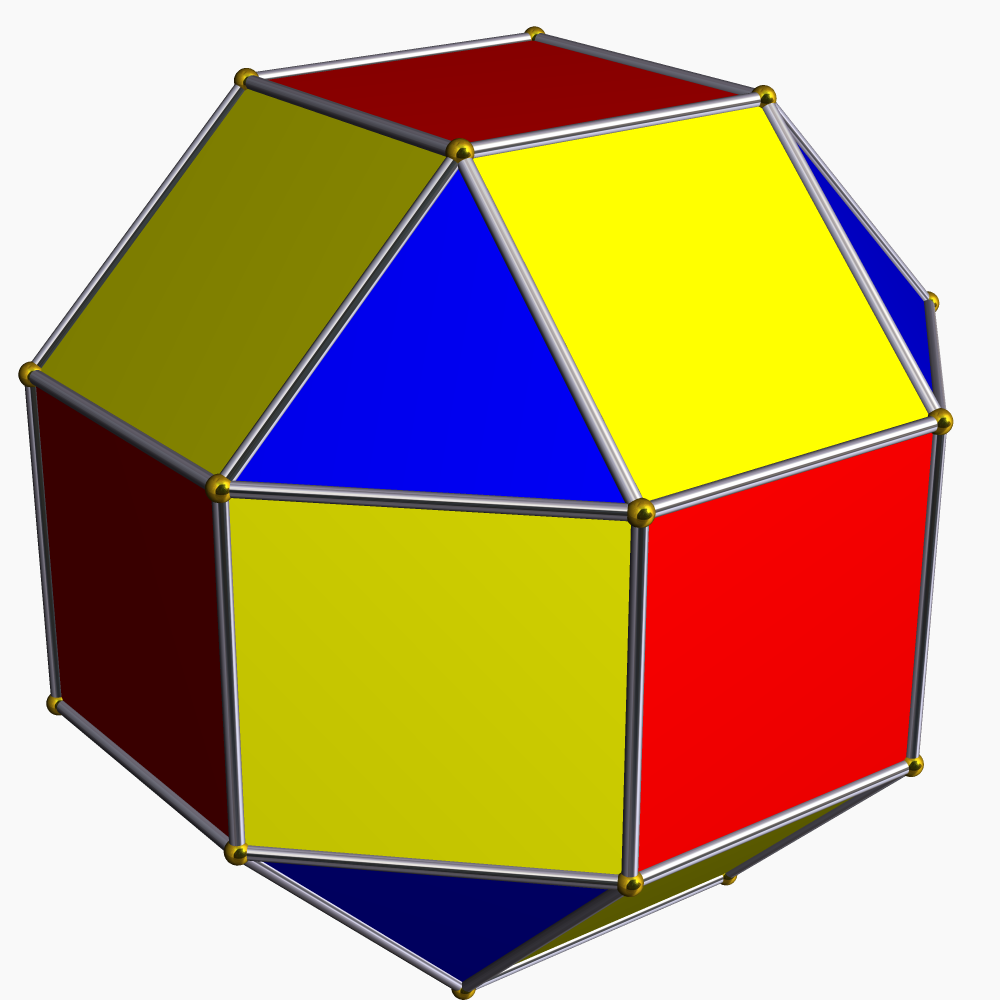
\includegraphics[width=0.9\linewidth]{Small_rhombicuboctahedron.png}
\caption{\small "Small rhombicuboctahedron" by Tomruen - \url{http://en.wikipedia.org/wiki/Image:small_rhombicuboctahedron.png.}}
\end{figure}
\end{column}
\end{columns}
\end{block}

\begin{block}{\LARGE\textbf{State of the Code}}
Currently my code is capable of advancing particle histories for the model problem.
No tally has yet been implemented.
\end{block}

\end{column}

\begin{column}{0.36\textwidth}

\begin{block}{\LARGE\textbf{MPI Shared Memory Allocation}}
Shared memory with MPI must be specially allocated with a calls to MPI functions.
Several steps are required to create and access this memory.
First, a MPI communicator for each group of shared memory processes must be created.

e.g.
\begin{lstlisting}
MPI_Comm comm = MPI_COMM_WORLD;
MPI_Comm shmcomm;
MPI_Comm_split_type(comm, MPI_COMM_TYPE_SHARED, 0, MPI_INFO_NULL, &shmcomm);
\end{lstlisting}
Then the shared memory must be allocated.

e.g.
\begin{lstlisting}
MPI_Aint size;
int disp_unit = sizeof(double);
double *shptr;
MPI_Win shwin;
MPI_Win_allocate_shared(size, disp_unit, MPI_INFO_NULL, shmcomm, &shptr, &shwin);
\end{lstlisting}
To get access to the shared memory region each process in the group must query the leading
memory address of the memory block.

e.g.
\begin{lstlisting}
MPI_Win_shared_query(shwin, 0, &size, &disp_unit, &shptr);
\end{lstlisting}
\end{block}

\begin{block}{\LARGE\textbf{MPI\_Accumulate}}
MPI\_Accumulate is a special function that allows each process to add a contribution to
a shared memory region in a safe way.

The MPI standard defines this function with:
\begin{lstlisting}
int MPI_Accumulate(const void *origin_addr,
 int origin_count, MPI_Datatype origin_datatype,
 int target_rank, MPI_Aint target_disp,
 int target_count, MPI_Datatype target_datatype,
 MPI_Op op, MPI_Win win);
\end{lstlisting}
\end{block}

\begin{block}{\LARGE\textbf{Ongoing Work}}
Implementing the shared memory tally is an ongoing process.
This work will need to be completed before conclusions can be drawn about the effectiveness
of shared memory tallies.
\end{block}

\end{column}

\end{columns}

\end{frame}

\end{document}